\section{Outcomes and Results}

Following classes and blocks were desingned as part of this project. These can be installed as an Out of Tree module in GNU Radio. The source can be downloaded from \cite{gr-ldpc}
   \begin{itemize}
    \item Class for GF$\left(2\right)$ Vector arithmetic.
    \item Class for GF$\left(2\right)$ Matrix arithmetic.
    \item Class for accessing LDPC codes in ``alist-file''\cite{alist} format.
    \item Class for holding an LDPC code.
    \item Class for message passing mechanisms for BSC and AWGN channels.
    \item LDPC Encoder block.
    \item LDPC Decoder blocks, for both float inputs and byte inputs.
    \item Two algorithms for construction of LDPC codes
   \end{itemize}

   Tables~\ref{tab:biter} and \ref{tab:blocker} compares the performance of these blocks with uncoded BPSK. The plot of Bit error performance is in Figure~\ref{fig:berplot}
   The GNU Radio set up used in this experiment is shown in Figure~\ref{fig:blocks}
   
\begin{table}
\caption{Bit Error Rate Comparison}\label{tab:biter}
\begin{center}
 \begin{tabular}{| c | c | c | c | c |}
 \hline
  sigma & Errors (No code)	& BER (No Code)	& Errors (With LDPC)	& BER (With LDPC) 	\\ \hline
  0.3  	& 4338			& 0.0004338	& 0			& 0			\\ \hline
  0.4	& 61814			& 0.0061814	& 0			& 0			\\ \hline
  0.5	& 227228		& 0.0227228	& 31			& 3.1e-06		\\ \hline
  0.6	& 477744		& 0.0477744	& 65855			& 0.0065855		\\ \hline
  0.7	& 765326		& 0.0765326	& 572393		& 0.0572393		\\ \hline
  0.8	& 1055848		& 0.1055848	& 968856		& 0.0968856		\\ \hline
  0.9	& 1332039		& 0.1332039	& 1291208		& 0.1291208		\\ \hline
  1.0	& 1585653		& 0.1585653	& 1565803		& 0.1565803		\\ \hline
 \end{tabular}
\end{center}
 \caption*{The performance of a (3, 6) regular LDPC code with $N = 96, K = 50,$ and $M = 48$}
\end{table}

\begin{table}
\caption{Block Error Rate Performance} \label{tab:blocker}
\begin{center}
 \begin{tabular}{| c | c | c | c | c |}
 \hline
  sigma & Errors (No Code)	& BER (No Code)	& Errors (With LDPC)	& BER (With LDPC) 	\\ \hline
  0.3  	& 3898			& 0.196461	& 0			& 0			\\ \hline
  0.4	& 18938			& 0.954488	& 0			& 0			\\ \hline
  0.5	& 19840			& 0.999994	& 0			& 0			\\ \hline
  0.6	& 19841			& 1.0		& 17			& 0.0008568		\\ \hline
  0.7	& 19841			& 1.0		& 19841			& 1.0			\\ \hline
 \end{tabular}
 \end{center}
 \caption*{The performance of an LDPC code generated using PEG with $N = 1008, K = 504,$ and $M = 504$}
\end{table}

  \begin{figure}
  \centering
   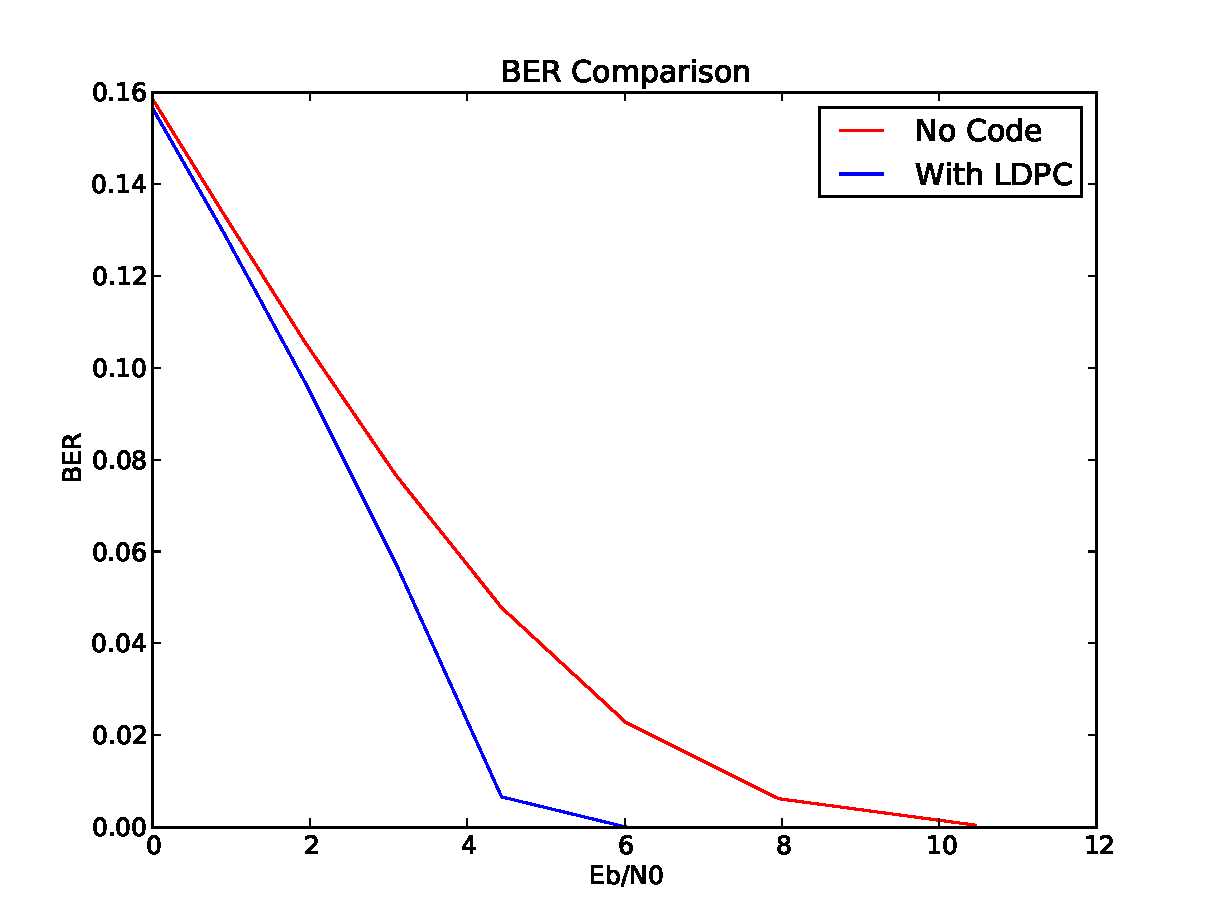
\includegraphics[scale = 0.5]{ber_plot.pdf}
   \caption{BER plot corresponging to Table~\ref{tab:biter}}
   \label{fig:berplot}
  \end{figure}

  \begin{figure}
  \centering
   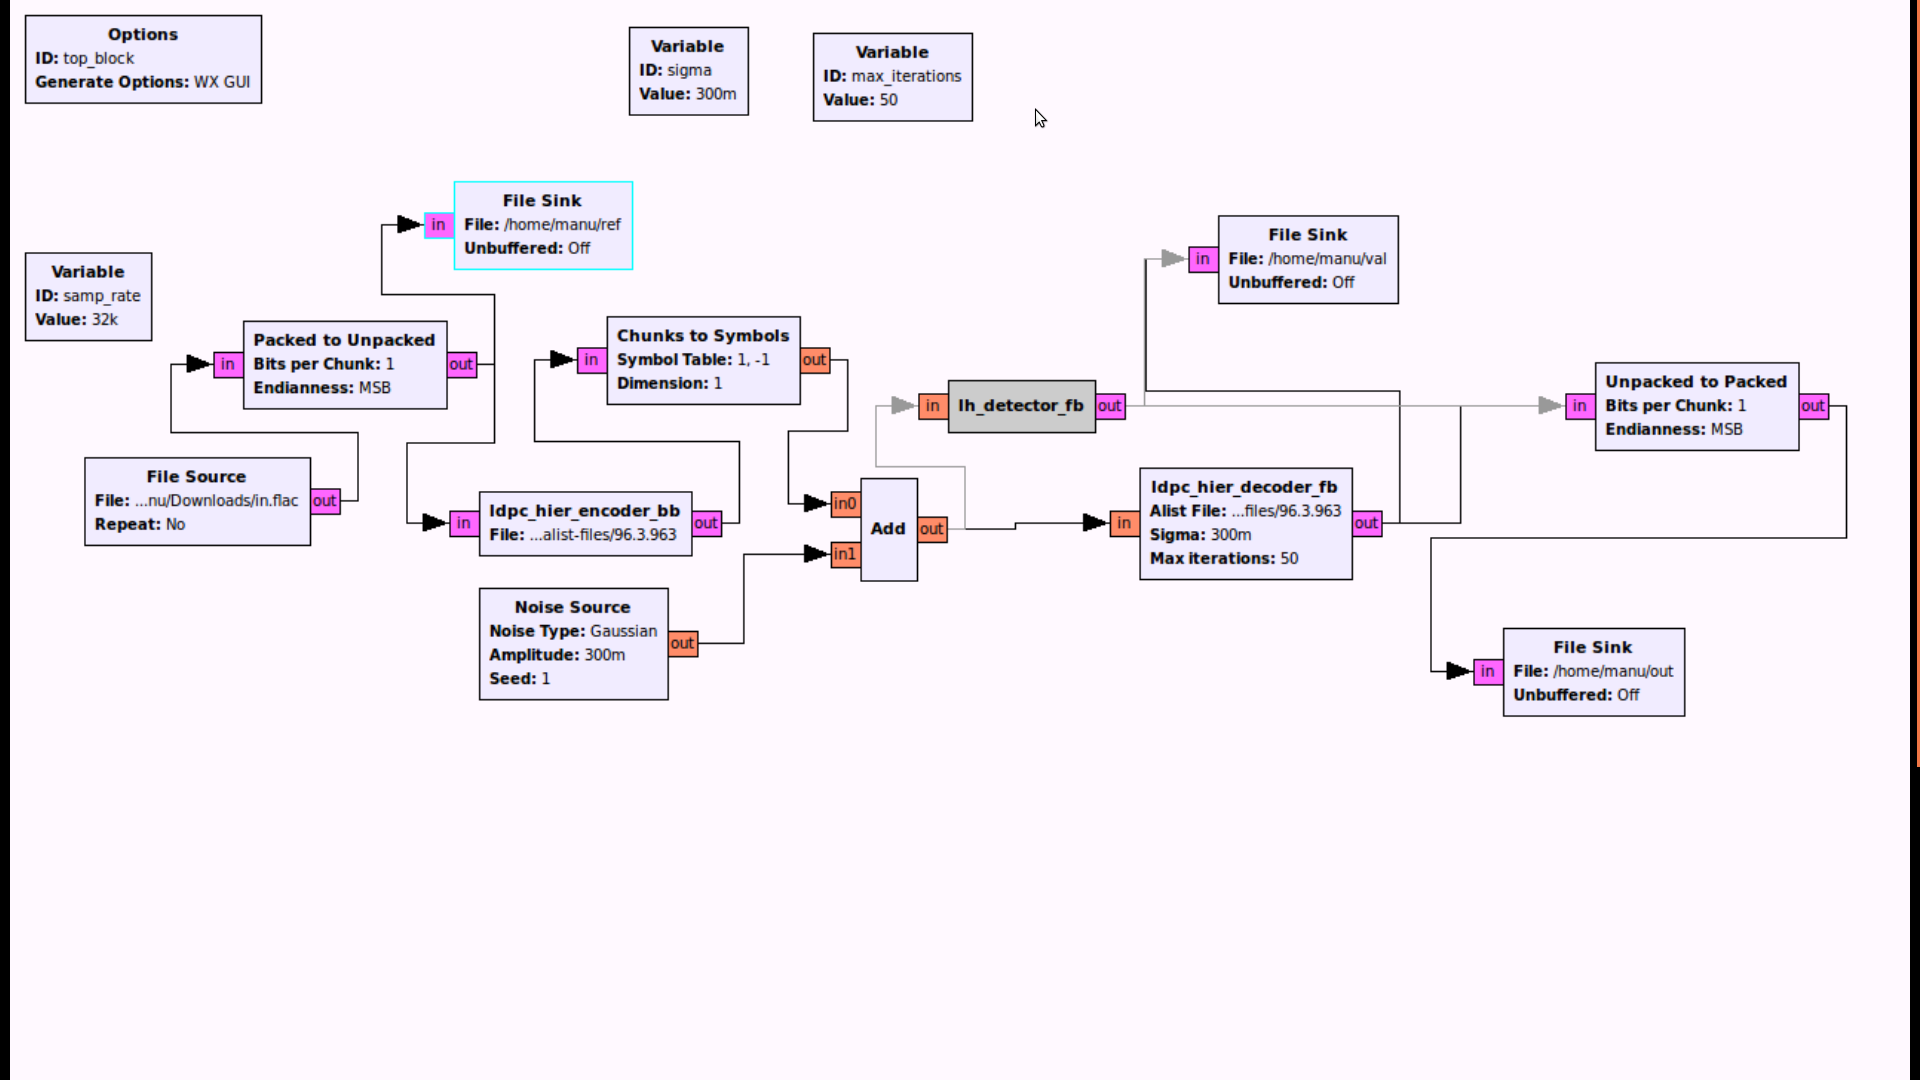
\includegraphics[scale = 0.2]{ldpc.png}
   \caption{GNU Radio block diagram} 
   \label{fig:blocks}
  \end{figure}